% siminos/CLE/movingFrames.tex
% $Author: siminos $ $Date: 2009-12-19 02:59:14 +0100 (Sat, 19 Dec 2009) $

The \mframes, introduced by G. Darboux and systematized by \'E. Cartan\rf{CartanMF},
can be thought of as generalization of the Frenet-Serret comoving frame.
The \Mframes\ can be used to generate functionally independent invariant coordinates
for the action of a group $\Group$ on a manifold $\Manif$ under
very general assumptions.  Here we will describe how, and to what extend,
the invariants thus generated can be utilized for symmetry reduction in 
high-dimensional flows. Our presentation draws from the reformulation of the \mframes\ 
by Fels and Olver\rf{FelsOlver98,FelsOlver99} but our emphasis is on the implementation
of the method as a geometrical, and therefore linear, operation that can be efficiently
implemented even in higher-dimensional flows, rather than in the explicit 
determination of invariant functions as in \refref{FelsOlver98,FelsOlver99}. 

The main idea behind \mframes\ is that we can, at least locally, 
map each point along any solution $\ssp(\tau)$ to a unique 
representative $\sspRed(\tau)$ of the associated
group orbit equivalence class, by a suitable rotation
\beq
\ssp(\tau) = \LieEl(\tau) \, \sspRed(\tau)
\,.
\ee{EquiTraj}
Equivariance implies the two points are equivalent.
In the `\mframes' the \reducedsp\ representative $\sspRed$
of a group orbit equivalence class is picked by slicing across the group orbits
by a fixed hypersurface.
%
%%%%%%%%%%%%%%%%%%%%%%%%%%%%%%%%%%%%%%%%%%%%%%%%%
\begin{figure}[h]
\begin{center}
 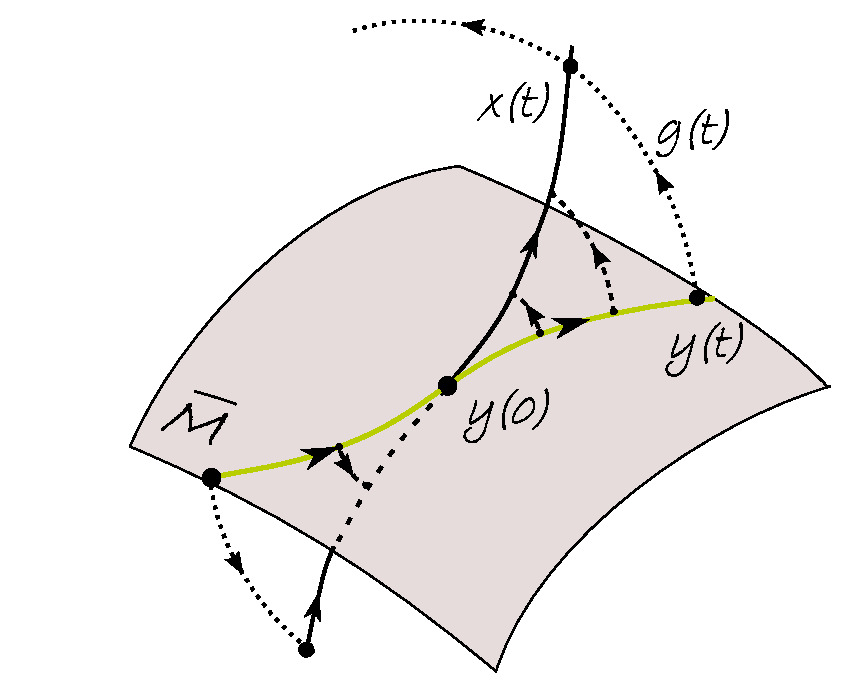
\includegraphics[width=0.5\textwidth]{../figs/ReducTraj}
\end{center}
\label{fig:ReducTraj}
\caption{
\Slice\ \pSRed\ is a Poincar\'e section \refeq{PCsectQ} for
group orbits (indicated by dotted lines here). The full
\statesp\ trajectory $\ssp(t)$ and and the \reducedsp\
trajectory $\sspRed(t)$ belong to the same group orbit
$\pS_{\ssp(t)}$ and are equivalent up to a group rotation
$\LieEl(t)$ \refeq{EquiTraj}.
}
\end{figure}
%%%%%%%%%%%%%%%%%%%%%%%%%%%%%%%%%%%%%%%%%%%%%%%%%%
%
\ES{move elsewhere: We start by describing how the
method works for a finite segment of the full \statesp\
trajectory.}

In the following it will be useful to introduce the
notion of a \emph{\slice}, an $(n-r)$-dimensional submanifold $K$
of $\Manif$ such that $K$ intersects all group orbits in an
open neighborhood of $\ssp \in K$ transversally and at most once. 
In other words, `\slice' is a Poincar\'e section
for group orbits. As is the case for the dynamical Poincar\'e sections,
in general a single \slice\ does not suffice to intersect all
group orbits of points in \pS. Fels and Olver\rf{FelsOlver99}
call a manifold $K$ that intersects \emph{all} group orbits a
\emph{regular cross-section}, and refer to a \slice\ as a local
cross-section. Here we prefer the term slice
to cross-section as the latter has a well established usage in the physics
literature.

Loosely speaking, one can construct a local {\csection} passing
through any point $x\in \Manif$ if the group orbits of \Group\
have the same dimension, \ie\ away from {\fixedsp s}
of continuous subgroups of \Group, see \refref{FelsOlver99} for
details.

The simplest {\em \slice\ condition} defines a linear \slice\ as a
$(d\!-\!N)$-dim\-ens\-ion\-al hyperplane \pSRed\ normal to
the $N$ group rotation tangents $\sliceTan{a}$ at point $\slicep
$:
\beq
(\sspRed - \slicep )^T \sliceTan{a} =0
    \,,\qquad
\sliceTan{a} = \groupTan_a(\slicep) = \Lg_a \, \slicep
\,.
\ee{PCsectQ}

%%%%%%%%%%%%%%%%%%%%%%%%%%%%%%%%%%%%%%%%%%%%%%%%%%
% computed by PCunrot.nb, then hand-drawn
% by dasbuch/book/FigSrc/xfig/PCunrot.fig
% then branched to dasbuch/book/FigSrc/xfig/ESunrot.fig
\begin{figure}
 \begin{center}
  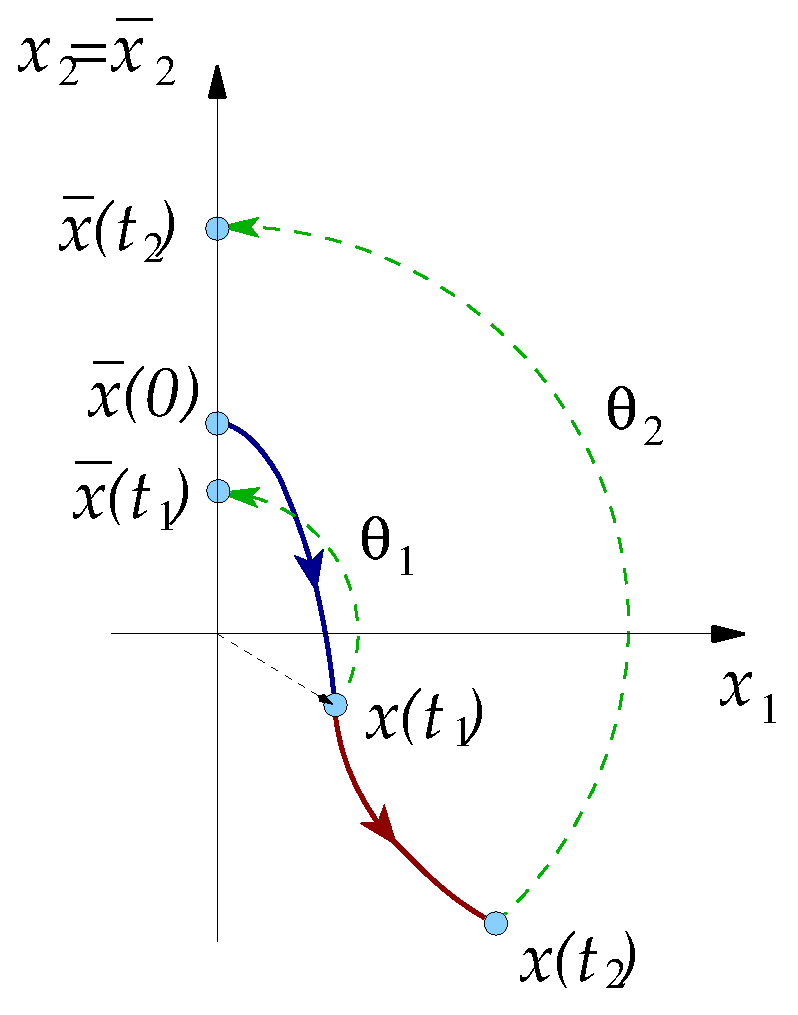
\includegraphics[width=0.5\textwidth]{../figs/ESunrot}
 \end{center}
 \label{fig:ESunrot}
 \caption{\Mframes\ for a flow $\SOn{2}$-equivariant under
\refeq{CLfRots} with \slice\ through $\slicep=(0,1,0,0,0)$,
group tangent $\sliceTan{}=(1,0,0,0,0)$. The clockwise
orientation condition restricts the \slice\ to half-hyperplane
$\sspRed_1=0,\;\sspRed_2>0$. A trajectory started on the
\slice\ at $\sspRed(0)$, evolves to a \statesp\ point with a
non-zero $\ssp_1(t_1)$. Compute the polar angle $\gSpace_1$
of $\ssp(t_1)$ in the $(\ssp_1,\ssp_2)$ plane. Rotate $\ssp(t_1)$
clockwise by $\gSpace_1$ to $\sspRed(t_1) =
\LieEl(-\gSpace_1)\,\ssp(t_1)$, so that the equivalent point
on the circle lies on the \slice, $\sspRed_1(t_1) =0$. Repeat
for all sample points $\ssp(t_i)$ along the trajectory.}
\end{figure}
%%%%%%%%%%%%%%%%%%%%%%%%%%%%%%%%%%%%%%%%%%%%%%%%%%


\ES{repeated?: In the following let $\Group$ be $N$-dimensional and act on a
$d$-dimensional manifold $\Manif$.}
\ES{dropped: Assume that for a given $\ssp\in\pS$ and a given \slice\
$\pSRed$ there exists} 

For group orbits intersected by a slice we can identify the unique group element
$\LieEl=\LieEl(\ssp)$ that rotates $\ssp$ into the slice,
$\LieEl\ssp = \sspRed \in \pSRed$. The map that
associates to a \statesp\ point $\ssp$ a Lie group action
$\LieEl(\ssp)$ is called a \emph{moving frame}.



As $\slicep^T \sliceTan{a} =0$ by the antisymmetry of
$\Lg_a$, the \slice\ condition \refeq{PCsectQ} fixes
$\gSpace$ for a given $\ssp$ by
    \index{post-processing}
\beq
0 = \sspRed^T  \sliceTan{a}
  %= \LieEl(\gSpace) \cdot \hat{\ssp}   \cdot \Lg \cdot \slicep
	=\ssp^T  \LieEl(\gSpace)^T \sliceTan{a}
\,,
\ee{PCsectQ1}
where $\LieEl^T$ denotes the transpose of $\LieEl$.
%    \PC{dropped ``
%    with the total shift $\gSpace(\tau)$ given by the sum
%    of stepwise rotations $\gSpace_j$.
%    }

\Mframes\ can be interpreted as a change of variables
\beq
\sspRed = \LieEl^{-1} \, \ssp
\,,
\ee{EquiTrajInvrs}
to a frame of reference in which condition
\refeq{PCsectQ1} is identically satisfied. Therefore the name
`moving frame.'

The \mframes\ is a post-processing method; trajectories are
computed in the full \statesp, then rotated into the \slice\
whenever desired, with the \slice\ condition easily
implemented. The \slice\ group tangent \sliceTan\ \, is a given
vector, and $\LieEl(\gSpace)\,\ssp$ is
another vector, linear in $\ssp$ and a function of group
parameters $\gSpace$. Rotation parameters $\gSpace$ are
determined numerically, by a Newton method, through the \slice\
condition \refeq{PCsectQ1}.

\refFig{fig:PCunrot} illustrates the \mframes\ for an
$\SOn{2}$ \slice\ normal to the $\ssp_2$ axis.
\index{SO(2)@\SOn{2}}
Looks innocent, except there is nothing to
prevent a trajectory from going through $(x_1,x_2)=(0,0)$,
and what $\gSpace$ is one to use then? We can always chose a
finite time step that hops over this singularity, but in the
continuous time formulation we will not be so lucky.
    \PC{add example here}

How does one pick a \slice\ point $\slicep$? A generic point
$\slicep $ not in an invariant subspace (on the \cLe\ $z$
axis, for example) should suffice to fix a \slice.
% for example a point on an \reqv\ group orbit,
% $\slicep  = \ssp_{\REQV{}1}$.
The rules of thumb are much like the ones for picking
Poincar\'e sections, \refsect{s:bestPoinc}. The intuitive
idea is perhaps best visualized in the context of fluid
flows. Suppose the flow exhibits an unstable coherent
structure that --approximately-- recurs often at different
spatial dispositions. One can fit a `template' to one
recurrence of such structure, and describe other recurrences
as its translations. A well chosen \slice\ point belongs to
such dynamically important equivalence class (\ie, group
orbit).
% We shall show in \refsect{sect:MovFrameODE} that
A \slice\ is locally isomorphic to $\pS/\Group$, in an open
neighborhood of $\slicep$. As is the case for the dynamical
Poincar\'e sections, in general a single \slice\ does not
suffice to reduce $\pS \to \pS/\Group$ globally.

\ES{re-insert?: To construct a moving frame, let $K\subset\Manif$ be a {\csection}. For $x\in \Manif$, let
$\LieEl=\rho(x)$ be the unique group element that maps $x$
to the {\csection}: $g x = \rho(x) x\, \in K$. Then
$\rho:\Manif\rightarrow \Group$ is a right moving frame\rf{FelsOlver98}.
}

\subsection{Coordinate {\csection s} and explicit invariants}

By proper choice of the {\csection} condition it is possible to
explicitly generate invariant variables for the group action.

A {\csection} $K$ can be defined by means of level sets of
functions $K_i(x)=c_i$, where $x\in V$ and $i=1,\ldots,r$. If
the $K_i(x)$ coincide with the local coordinates $x_i$ on the
manifold $V$, \ie~$K_i(x)=x_i$, then we call $K$ a
\emph{coordinate \csection}.


Once a coordinate cross-section
$K=\{x_1=c_1,\ldots,x_r=c_r\}$ is defined by the first $r$
coordinates (relabel coordinates as necessary),
we write the group transformations as
\beq
	\overline{x}= g \cdot x = w(g,x)\,.
	\label{eq:transNorm}
\eeq
Equating the first $r$ components of the function $w$ to the
constants in the definition of the {\csection} $K_i(x)=c_i$
yields the \emph{normalization equations} for $K$:
\beq
	\overline{x}_1=w_1(g,x)=c_1,\ldots,\overline{x}_r=w_r(g,x)=c_r\,.
	\label{eq:normalization}
\eeq
The normalization equations \refeq{eq:normalization}
can always be solved\rf{FelsOlver99} for the group parameters in terms of
$x$, yielding the moving frame associated with $K$:
$\LieEl=\LieEl(x)$. Substitution of the moving frame equation back
in \refeq{eq:transNorm} will yield the $n-r$
\emph{fundamental invariants}, that is functionally independent
invariants that can be used as a basis in which any other invariant
can be expressed. Thus the fundamental invariants serve to distinguish
group orbits in the neighborhood of the {\csection}, \ie~two points
lie on the same group orbit if and only if all fundamental invariants
agree. For proof \cf~\refrefs{FelsOlver98,FelsOlver99}.

Invariants generated by \mframes\ can be used in the same manner as a Hilbert
polynomial basis for symmetry reduction, by projecting $d$-dimensional trajectories
to $(d-N)$-dimensional variables. The fact that a moving frame exists
only where group orbits have the same dimension is not as severe a restriction
as it might seem. This condition fails on a \fixedsp\ of a continuous subgroup
of \Group\ but, as we have seen in \refsect{s:symDyn}, {\fixedsp s} are flow-invariant.
Therefore, one can always hope to cover the reduced space with properly chosen {\csection s}.
Nevertheless, as we will see in next section, coordinate {\csection s} are not an optimal
choice for common actions of \SOn{2} on truncations of PDEs, such as in the \cLe\ example.





\subsection{\label{sec:CLeMF}Moving frame invariants for \cLe}


%%%%%%%%%%%%%%%%%%%%%%%%%%%%%%%%%%%%%%%%%%%%%%%%%%%%%%%%%%%%%%%%
\begin{figure}[ht]
\begin{center}
  (\textit{a})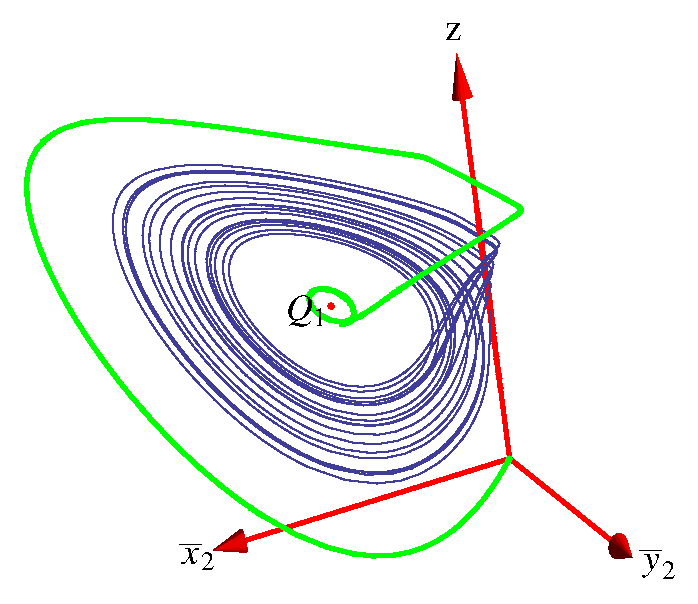
\includegraphics[width=0.35\textwidth]{../figs/CLEmfXYZ}
~~~~(\textit{b})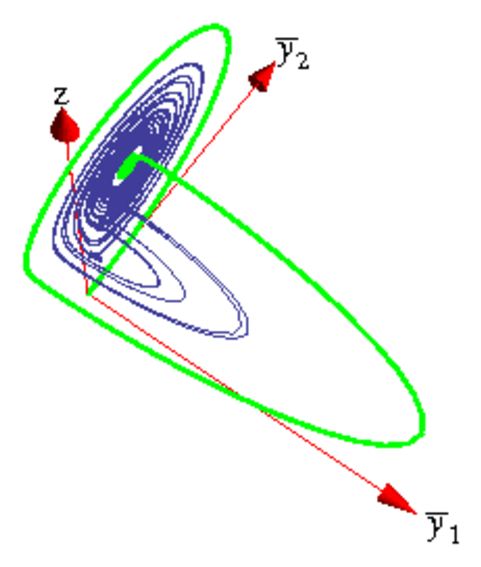
\includegraphics[width=0.35\textwidth]{../figs/CLEmfYYZ}
\end{center}
\caption{ \Statesp\
portraits of \cLe\ dynamics for $e=1/10$, $\ImrCLor=0$
in \reducedsp. Projecting on invariants given in \refeq{eq:invLaser}.
    }
\label{fig:CLEmf}
\end{figure}
%%%%%%%%%%%%%%%%%%%%%%%%%%%%%%%%%%%%%%%%%%%%%%%%%%%%%%%%%%%%%%%%

In this section we illustrate symmetry reduction through
the use of invariants computed
with the moving frame method in the example of \cLe.
The $z$-axis is the \fixedsp\ of \SOn{2} acting by
\refeq{eq:SO2act} on \Rls{5}. Therefore we can define
a coordinate {\csection} on $\Rls{5}\backslash\{x_1=x_2=y_1=y_2=0\}$
by, for instance,
\beq\label{eq:CLEsliceSO2}
x_1=0,\,x_2>0\,.
\eeq
We can now construct a moving frame for the action
\refeq{eq:SO2act} of $\SOn{2}$ as follows. We write out
explicitly the group transformations:
\begin{subequations}\label{eq:CLEnorm}
\begin{align}
 	\overline{x}_1 &= x_1 \cos\theta - x_2 \sin\theta\label{eq:CLEexplSO2a}\cont
	\overline{x}_2 &= x_1 \sin\theta + x_2 \cos\theta\label{eq:CLEexplSO2b}\cont
	\overline{y}_1 &= y_1 \cos\theta - y_2 \sin\theta\label{eq:CLEexplSO2c}\cont
	\overline{y}_2 &= y_1 \sin\theta + y_2 \cos\theta\label{eq:CLEexplSO2d}\cont	
	\overline{z} &= z\,.
\end{align}
\end{subequations}
We set $\overline{x}_1=0$ and solve
\refeq{eq:CLEexplSO2a} for the group parameter to obtain the moving frame
\beq
	\theta=\tan^{-1}\frac{x_1}{x_2}
	\label{eq:CLEmf}
\eeq
which brings any point  back to the {\csection}.
Here it is important that
$\tan^{-1}$ distinguishes quadrants in the $(x_1,x_2)$ plane to ensure that the
transformation results in the correct geometric
interpretation, \ie\ to ensure $x_2>0$.
Substituting \refeq{eq:CLEmf} in the remaining equations \refeq{eq:CLEnorm} we
get the invariants
\beq
\begin{split}
	\overline{x}_2 &=  r_1 = \sqrt{x_1^2+x_2^2} \cont
	\overline{y}_1 &= {(x_2 y_1-x_1 y_2)}/{r_1}\cont
	\overline{y}_2 &= {(x_1 y_1+x_2 y_2)}/{r_1}\cont	
	\overline{z} &= z\,.
	\label{eq:invLaser}
\end{split}
\eeq
    \ES{The solution $\theta = 2
    \tan^{-1}\frac{-x_2+\sqrt{x_1^2+x_2^2}}{x_1}$ was
    returned by Mathematica. If we use $\theta =
    \tan^{-1}\frac{x_2}{x_1}$ without taking care of the
    quadrant our results are multiplied by $sgn(x_2)$.}
Note the relation to the invariant polynomials
\refeq{eq:ipLaser} and also that no syzygy is present.

Note that the invariants are not well defined
in the $x=x_1+i x_2 \to 0$ limit.
Using $x=r_1\, e^{i\phi_1}\,,\, y=r_2\, e^{i\phi_2}$ we can write
\ES{dropped: for instance, $x_2 y_1-x_1 y_2 = r_1 r_2 \sin(\phi_1-\phi_2)$
and thus}
\beq
  \begin{split}
	  \overline{x}_2 &= r_1 \cont
	  \overline{y}_1 &= r_2\sin(\phi_1-\phi_2)\cont
	  \overline{y}_2 &= r_2\cos(\phi_1-\phi_2)\cont	
	  \overline{z} &= z\,.
	  \label{eq:invLaserPolar}
  \end{split}
\eeq
Therefore, for any given $y$ (therefore also for given $\phi_2$),
the limit of $\overline{y}$ for $x \rightarrow 0$
does not exist, as the above expression depends on the direction
on the complex $x$-plane along which we approach zero.
\ES{does not belong here:
In terms of projecting dynamics
on variables \refeq{eq:invLaser} (or applying the equivalent
procedure of rotating points back to the \slice) this means that
we need to take into account the direction along which
we approach zero and use the `angle
of descent' as the angle with which we rotate points back to the \slice, if such
points have exactly $x=0$.
	}
Note that the invariants are not defined on
the subspace $U_S$ defined by $x_1=x_2=0$ even though the
group action is non-regular only in a subset of $U_S$, the
$z$-axis $x_1=x_2=y_1=y_2=0$ which is the \fixedsp\ of \SOn{2}.
In the spirit of \refref{GL-Gil07b} the transformations \refeq{eq:invLaser}
can therefore be characterized as non-optimal, in the sense
that we have singularity in a proper superset of $\Fix{\SOn{2}}$.
    \PC{``proper superset''? Il cano no parla questa lingua}
The reason the transformations fail on $U_S$ and not only on the $z$-axis
can be traced back to the way we construct the moving frame. The action
of the group can be thought of as a direct sum of irreducible
actions and the corresponding invariant (linearly irreducible)
subspaces are the $(x_1,\,x_2)$ and $(y_1,\,y_2)$
planes.
%PC OK \ES{Not sure if planes is acceptable term here.}.
Since irreducible subspaces are by definition group-invariant
implies that we could define a moving frame in any one of them
independently. The singular subspace would then be determined
by the fixed points of group action in this subspace alone.
For instance, by choosing an angle in the $(x_1,\,x_2)$ irreducible subspace
as the moving frame map, the singular set is the point
$x_1=x_2=0$ in this irreducible subspace. Going back to the full
$5$-dimensional space the singular set of the transformations
is still given by $x_1=x_2=0$.
%}

While a singularity in $\Fix{\SOn{2}}$ cannot be reached by generic orbits
as {\fixedsp s} are flow invariant, the same is not true for {\fixedsp s}
of irreducible representations of the group action\ES{make sure!!!}.
The fact that trajectories of \cLf\ in \reffig{fig:CLEmf} stay away from $r_1=0$ is therefore
fortuitous.

It is instructive to write \cLe~\refeq{eq:CLe} in the
variables \refeq{eq:invLaser}. This is achieved by using the
chain rule \refeq{ChainRul} and expressing the result in
terms of variables \refeq{eq:invLaser}. The equations now
read
\beq
\begin{split}
\dot{\overline{x}}_1 &= 0\,\\
\dot{\overline{x}}_2 &=-\sigma  \left(\overline{x}_2-\overline{y}_2 \right)\,,\\
\dot{\overline{y}}_1 &=-\overline{y}_1- \left(e+\sigma\frac{\overline{y}_1}{\overline{x}_2} \right)\overline{y}_2\,,\\
\dot{\overline{y}}_2 &=(\RerCLor -z)\overline{x}_2+\left(e+\frac{\sigma  \overline{y}_1}{\overline{x}_2}
\right) \overline{y}_1-\overline{y}_2\,,\\
\dot{z} &=\overline{x}_2 \overline{y}_2-b z\,.
\end{split}
\eeq
We again observe the singularity as
$\overline{x}_2=r_1\rightarrow 0$.

The projections in \reffig{fig:CLEmf} reveal more about the
topology of the attractor but also present large ``jumps."
Note that the invariants \refeq{eq:invLaser} are related to
the invariant polynomials \refeq{eq:ipLaser} by division by
$\sqrt{x_1^2+x_2^2}$. This is the reason we get a clearer
visualization of the dynamics: All invariants scale
dimensionally as the original coordinates. At the same time
division by $\sqrt{x_1^2+x_2^2}$ causes the jumps in the
$\overline{y}$ components whenever the magnitude of $x$ comes
close to zero.

\PublicPrivate{}{
\ES{I think I might drop this part of the section, as it is a simple but
ad-hoc  modification. I will have to make sure that return map
figures are not completely elliminated from this section though.}
Geometrically we can interpret the jumps in the
$\overline{y}$ coordinates as follows: We have chosen to
measure angle on one of the irreducible subspaces of \SOn{2},
the $x$-plane, and project the dynamics on orbit space by
counter-rotating in both irreducible subspaces (the $x$- and
$y$-plane.) As long as a trajectory traces one lobe of the
Lorenz attractor the angle varies slowly and no problem
occurs. When a trajectory changes quadrant in the $x$-plane
to visit the almost opposite lobe (due to detuning we do not
visit the lobe related by rotation by $\pi$, in reality no
such thing exists) we get a rapid change in angle as the
trajectory passes close to the origin. In the $y$-plane we do
not necessarily change quadrant. Call $\Delta \theta_x$ and
$\Delta\theta_y$ the change in angle in the $x$- and
$y$-plane respectively, when the trajectory changes quadrant
in the $x$ plane. We always reduce to \reducedsp\ by
correcting by $-\Delta\theta_x$ instead of correcting by the
smallest angle.
}%end \PublicPrivate.

% Since $x$ cannot vanish
% The problem is mostly aesthetical in the present case,
% but for \KS\ system it will be important to prevent
% the denominator from vanishing.
%     \ES{Here I have a hunch that the denominator cannot
%     vanish but I can't prove it}
\PublicPrivate{}{
We observe that dynamics cannot enter $\Fix{\SOn{2}}$, \ie\
the $z$-axis, since {\fixedsp s} are flow invariant. Since
\SOn{2} representation in the \cLe\ example is a direct sum
of irreducible representations we cannot take more than one
irreducible subspace into account when setting up the
normalization equations, at least not in a convenient way. We
can however restore democracy between modes and extend
validity of the transformations to any point where the group
acts freely, by modifying the invariants as follows:
\beq
\begin{split}
	\overline{x}_2 &= (x_1^2+x_2^2)/r \cont
	\overline{y}_1 &= -(x_2 y_1-x_1 y_2)/r\cont
	\overline{y}_2 &=(x_1 y_1+x_2 y_2)/r\cont
	\overline{z} &=z\cont
	r &= \sqrt{x_1^2+x_2^2+y_1^2+y_2^2}
    \,.
	\label{eq:invLaser2}
\end{split}
\eeq
This set of invariants lacks a geometric interpretation\ES{or
does it?} but results in much cleaner phase portraits, \cf
\reffig{fig:CLEinv}.


%%%%%%%%%%%%%%%%%%%%%%%%%%%%%%%%%%%%%%%%%%%%%%%%%%%%%%%%%%%%%%%%%%
\begin{figure}[ht]
\begin{center}
  (\textit{a})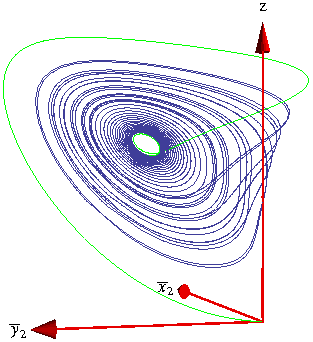
\includegraphics[width=0.35\textwidth]{../figs/CLEinvXYZ}
~~~~(\textit{b})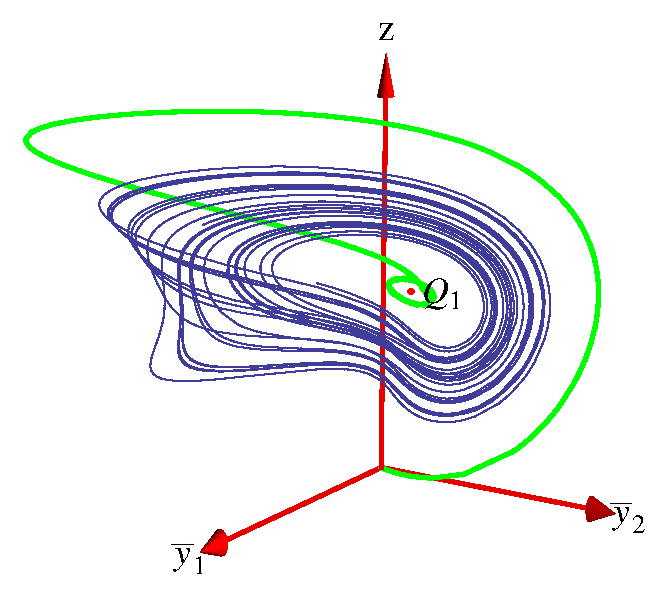
\includegraphics[width=0.35\textwidth]{../figs/CLEinvYYZ}
\end{center}
\caption{
\Statesp\ portraits of \cLe\ dynamics for $e=1/10$,
$\ImrCLor=0$ in \reducedsp. Projecting on invariants given in
\refeq{eq:invLaser2}.
    }
\label{fig:CLEinv}
\end{figure}
%%%%%%%%%%%%%%%%%%%%%%%%%%%%%%%%%%%%%%%%%%%%%%%%%%%%%%%%%%%%%%%%
\marginpar{Fetch return map figure using unmodified invariants.}

%%%%%%%%%%%%%%%%%%%%%%%%%%%%%%%%%%%%%%%%%%%%%%%%%%%%%%%%%%%%%%%%%%
\begin{figure}[ht]
\begin{center}
%   (\textit{a})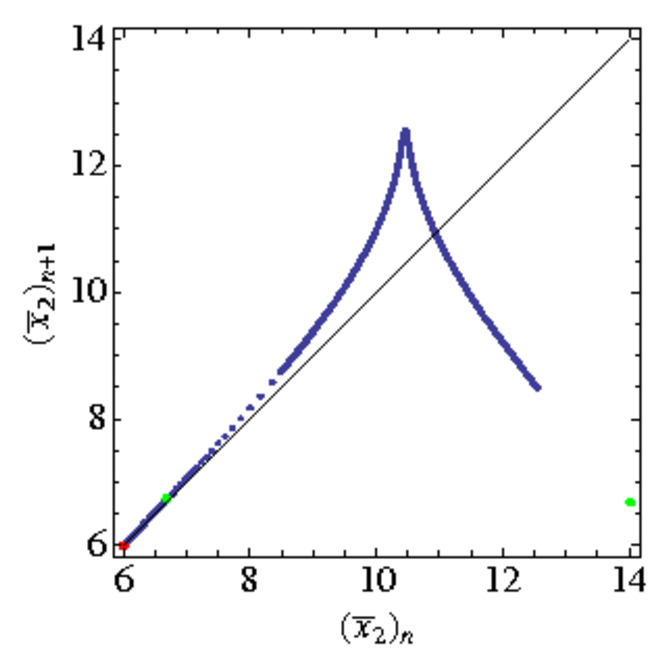
\includegraphics[width=0.35\textwidth]{../figs/CLEinvRMx2}
%  ~~~~(\textit{b})
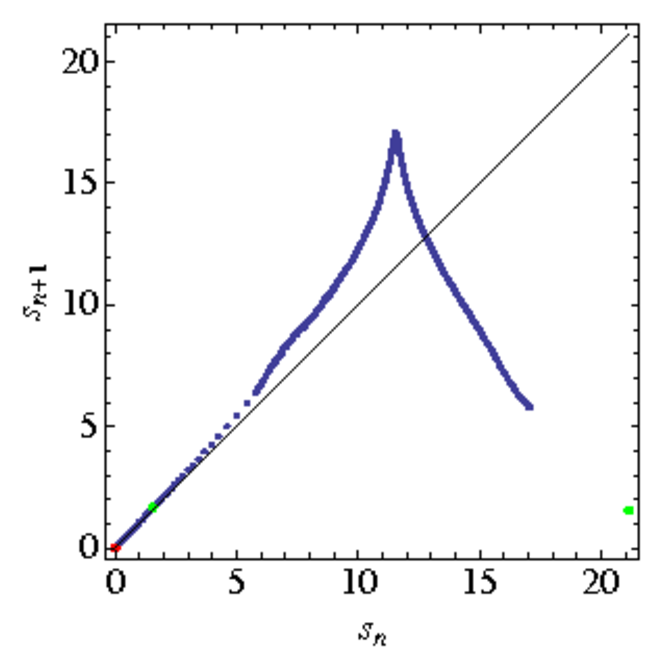
\includegraphics[width=0.35\textwidth]{../figs/CLEinvRM}
\end{center}
\caption[Return map for Complex Lorenz flow]{
Return map to the \Poincare\ surface of section
$\overline{x}_2=\overline{y}_2$ for \cLe\ with $e=1/10$,
$\ImrCLor=0$, projecting on invariants given in
\refeq{eq:invLaser2}. The return map coordinate is the
Euclidean length along the \Poincare\ section of the unstable
manifold of $E_1$.
    }
\label{fig:CLEinvRM}
\end{figure}
%%%%%%%%%%%%%%%%%%%%%%%%%%%%%%%%%%%%%%%%%%%%%%%%%%%%%%%%%%%%%%%%
} %end PublicPrivate
